\section{Framework}
The framwork presented in this work allows the user to \textbf{customize} the elements to be used in the design of the \textit{Custom Processor} and \textit{Memory System}, \textbf{explore} custom architectures automatically generated for a given application and \textbf{predict} area, power and latency of such architectures. Figure~\ref{fig:framework} gives an overview of the modules contained in the framework. The framework takes two inputs, the \textit{Configuration Parameters} - described in~\ref{ssec:conf_param} - and an \textit{Application} - detailed in~\ref{ssec:app}. A set of hardware architectures, behaviorally equivalent to the input application, is automatically generated by the framwork. The output is the area, power and latency tradeoff of such architectures. The generated hardware architectures can be used to generate an RTL implementation using the \textit{architectural templates} described in~\ref{sec:arch_template}.
The framework is composed by three modules. The first module - \textit{L2 Model} - models the transfer of the input data between the \textit{Layer 2} memory and the \textit{Layer 1} memory. The \textit{Data Dependency Analysis} performs static analysis on the input application. The last module, \textit{Design Space Exploration}, uses the information extracted by the previous step to procedurally generate hardware architectures.
The rest of this section will describe more in detail the inputs and modules of the framework.
\begin{figure}[tb] 
\centering
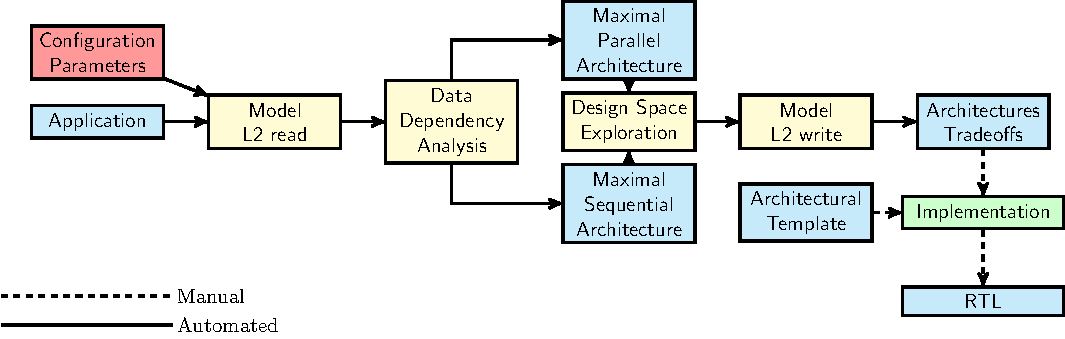
\includegraphics[width=\columnwidth]{images/framework.pdf}
\caption{\small Diagram of the Framework presented in this work.}
\label{fig:framework}
\end{figure}

\subsection{Application}
\label{ssec:app}
The framework performs exact data dependency analysis on the application. This entails that the behaviour of the application needs to be completely specified at compile-time and independent from the input data. Streaming applications meet these requirement and can be analyzed by our framework. Listing~\ref{lst:matrixvec} shows the application source code that will be used for the rest of this paper. The language that the framework currently supports is C/C++, however the framework uses the LLVM Intermediate Representation CITATION NEEDED, so the support for other languages can be easily added.
\begin{lstlisting}[language=C, caption={Example of input application, C implementation of a matrix vector multiplication.}, label={lst:matrixvec}]
void matrix_vec_kernel(int *A,int *B, int *C){
    int sum;
    for(int i=0;i<DIM2;i++){
        sum=0;
        for(int j=0;j<DIM1;j++){
            sum+=A[i*DIM1+j]*B[j];
        }
        C[i]=sum;
    }
}
\end{lstlisting}

\subsection{Configuration Parameters}
\label{ssec:conf_param}
The second input to the framework is a configuration file. The Configuration file contains a description of the different component to be used in the realization of the hardware architecture, an example is shown in Listing~\ref{lst:conf_file}. Using this file the user can specify the process technology to be used - e.g. 16nm, 28nm - the clock frequency of Layer 1 memory, Layer 2 memory and Custom Processor. The user can moreover specify the datawidth used by the different operators - e.g. multipliers, adders-, and by the Layer 1 and Layer 2 memory. 
Detailed information requred to model the Layer 2 burst accesses are as well contained in this file: the setup latency for write/read accesses, the type of Layer 2 memory to be used -e.g. MRAM, SRAM etc..- and the size of the Layer 2 memory.
\textbf{TODO}: describe the L1 memory model ( linear model that extrapolate area/power/energy using the depth as a variable to fill in missing values in the database)
\begin{lstlisting}[language=json, caption={Example of input configuration file}, label={lst:conf_file}]
{ 
   "resource_database": { 
	"technology": 16, 
	"clock_frequency": 1000, 
	"bitwidth_adder": 128, 
	"bitwidth_multiplier": 64, 
	"bitwidth_register_file": 128, 
	"type_l2": "tt1v1v85c", 
	"technology_l2": 16, 
	"clock_l2": 800, 
	"bitwidth_l2": 32, 
	"depth_l2":2048, 
	"setup_write_latency_l2":2, 
	"setup_read_latency_l2":2 
   } 
}

\end{lstlisting}

\subsection{Layer 2 Read Model}
\label{ssec:l2_read_model}
The first operation performed by the framework is to compute the transfer time of the application input data from the \textit{Layer 2} memory to the \textit{Later 1} memory. An address in Layer 2 memory is given to the input element used by the application, different datastructures are placed in consecutive memory addresses. The entire data transfer is modeled as a single burst read operation to the \textit{Layer 2} memory (see BACKGROUND). The information required to compute the arrival clock time of each input element to the Layer 1 memory is extracted from teh \textit{Configuration Parameters} and performing static analysis on the input \textit{Application}.
Using such information  the exact clock at which each input elements arrives in the Layer 1 memory can be computed with:
$$
AClk_i = rSL + (L2Add_i+1) * (L1B/L2B) * (L1Clk/L2Clk)
$$

Where $AClk_i$ is the clock at which element i arrives to the Layer 1 memory, $rSL$ is the setup latency of a Layer 2 burst read, $L2Add_i$ is the offset of element i from the beginning of the burst access, $L1B$ is the data bitwidth of the Layer 1 memory, $L2B$ is the data bitwidth of the Layer 2 memory, $L1Clk$ is the clock frequency of the Layer 1 memory and $L2Clk$ is the clock speed of the Layer 2 memory.

\subsection{Data Dependency Analysis}
The \textit{Data Dependency Analysis} module performs three main operations. First, it extracts \textit{Data Dependency Graph} (DDG) from the application. Then, it schedules the DDG using the As Soon As Possible (ASAP) and As Late As Possible (ALAP) methodologies. Finally, it maps instructions in the DDG to hardware components - or Functional Units (FUs) - using a modified version of the \textit{Interval Partitioning} algorithm ADDCITATION.
%This next paragraph might be replaced with a reference
To extract the DDG from an application we use LLVM  and custom transformations. We first convert the input application code to its LLVM Intermediate Representation. We then transform the code into static single assignment (SSA) form and perform full-loop unrolling on all of the application loops. After these transformation there will be no control flow instructions in the application body and each variable will be defined only once. Following the chain of use and definition of the application variables is then possible to produce a Data Dependency Graph like the one shown in Figure ADDIMAGE. 
We further process the obtained DDG in the aim to reduce the lenght of the path between the input nodes and the output nodes. The reason is that the lenght of such paths is equivalent to the number of successive operations required to obtain the outputs which is connected to the latency of the application. Taking advantage of the commutativity of some operation we can transform a long sequence of operations into an equivalent shorter tree as shown in Figure ADDIMAGE.
%This next paragraph might be replaced with a reference, we are interested mainly in the concept of mobility
In the second step we apply the ASAP and ALAP scheduling methodologies to the generated DDG. These schedules will associate each node of the DDG to a clock cycle where the instruction is executed. We start by scheduling the input nodes of the DDG using the arrival clock time of their element, computed as explained in~\ref{ssec:l2_read_model}. This allows us to take into account the transfer time between the Layer 2 memory and Layer 1 memory. We then derive the minimal latency required to obtain the outputs of the application with the ASAP schedule: starting from the DDG input leafs each instruction node is scheduled as soon as its dependencies are resolved. 
Once a clock is assigned to the output leaf nodes of the DDG we can perform the ALAP scheduling: starting from the output leaf nodes each dependency node is scheduled as late as possible. After this second step, each node will then have an associated ASAP schedule and ALAP schedule. The difference between these two schedules is called \textit{mobility} of the node. The mobility of a node identifies an interval of clocks in which the instruction can be scheduled without changing the overall latency of the application.
The final step of the \textit{Data Dependency Analysis} module - described in~\ref{ssec:modified_interval_partitioning} - will allocate the DDG nodes to FU, using the nodes mobility to minimize the number of FUs of the final hardware architecture. 

\subsection{Modified Interval Partitioning}
\label{ssec:modified_interval_partitioning}
To generate an hardware architecture behaviorally equivalent to the input application and with the latency identified during the ASAP-ALAP scheduling, there are two main requirements. The first is that each instruction needs to be computed within its ASAP-ALAP interval. The second requirement is that instructions in the original DDG which are executed by the same FU cannot be scheduled at the same time.
Our Modified Interval Partitioning algorithm - based on the original greedy Interval Partitioning algorithm CITE - is able to generate hardware architectures from a DDG meeting the two requirements described above. The original Interval Partitioning problem addresses the issue of assigning a number of jobs, with known starting and ending time, to the minimum amount of resources ensuring that the jobs assigned to a resource do not overlap. To map the Interval Partitioning formulation to the allocation of instructions to FU, we need to consider application instructions as jobs and FUs as resources. 
There are however three main differences between our problem and the canonical Interval Partitioning. First, while in the original Interval Partitioning problems jobs are equivalent to each other and can be assigned to any resource, the instructions represent computations. For example a multiply instruction can only be assigned to a multiply FU. To address this issue, we divide our initial problem and we perform multiple time the Interval Partitioning, once per operation type. This ensures a correct allocation of the instruction to FUs performing the same operation. The second difference is due to the \textit{mobility} of our instructions. Each instruction does not have a predefined start and end time, like a job has in the original Interval Partitioning, but it has a time interval - derived with ASAP-ALAP - in which it can be scheduled and a fixed latency. Hence, the start time of an instruction might vary, but once this is fixed, its end time can be derived. The modified Interval Partitioning takes the mobility of an instruction into account allowing a given instruction to start at any time within its allowed interval. The last difference regards the dependencies between instructions. While the original jobs in the Interval Partitioning are intependent from each other, the instructions of an application need to be executed according to their dependencies. This is addressed by ensuring that a given instruction is allocated after its dependencies are allocated and by verifying that its starting time is scheduled after the ending time of its dependencies.
Listing~\ref{lst:modified_interval_partitioning} shows the pseudocode of our modified interval partitioning algorithm.
\begin{lstlisting}[language=C, caption={Example of input configuration file}, label={lst:modified_interval_partitioning}]
sort i in instructions by ASAP[i]
for each i in instructions
	allocated = False
	earliest_starting_time[i] = ASAP[i]
	if i has dependencies
		end_max_time = max end time among all dependencies of i
		earliest_starting_time[i] = end_max_time
	for each Functional Unit fu where type(fu) ==  type(i)
		if ALAP[i] >=  next_free_slot[fu]
			fu.instructions += [i]
			schedule[i] = max(earliest_start_time[i],next_free_slot[fu])
			next_free_slot[fu] = schedule[i] + latency[i]
			allocated = True
	if not allocated
		create new Functional Unit fu where type(fu) == type(i)
			fu.instructions += [i]
			schedule[i] = earliest_start_time[i]
			next_free_slot[fu] = schedule[i] + latency[i]

\end{lstlisting}

\subsection{Maximal Parallel Architecture and Maximal Sequential Architecture}
\subsection{Design Space Exploration}
\subsection{Layer 2 Write Model}
\subsection{Architecture Tradeoffs}

